\documentclass{article}

\usepackage{amsmath, amsthm, amssymb, fancyhdr, graphicx}
\graphicspath{{./images/}}
\pagestyle{fancy}
\lhead{DREAL Paper Reading: MV-GPT}
\begin{document}
\paragraph{Abstract Summary:} Multimodal Video Generative Pretraining (MV-GPT) is this paper's
novel framework for learning from unlabelled videos which can effectively be used for generative
tasks such as multimodal video captioning.

\begin{itemize}
    \item Trains a multimodal video encoder and a sentence decoder jointly.
    \item Leverages future utterances as additional text sources, proposes a bidirectional
        generation objective --- generate future utterances given present multimodal context,
        and the present utterance given future observations.
    \item Train an encoder-decoder model end-to-end to generate a caption from raw pixels and
        transcribed speech directly.
\end{itemize}

\paragraph{Introduction:} A long-standing goal of AI is the development of conversational multimodal
systems that can both reliably perceive the world and effortlessly communicate with humans. 

\paragraph{}Multimodal video captioning tests both abilities; a successful model must not only accurately
understand \emph{'multimodal'} streams of input video (including speech and video frames), but also 
generate coherent natural language descriptions of the content.

\paragraph{Motivation:}In the field of computer vision and language learning, there is a lack of
large-scale, manually annotated data. Annotating captions for videos is time intensive, expensive,
and subjective (low inter-annotator agreement).

\paragraph{}This is largely in contrast with image classification, where fully annotated datasets are
orders of magnitude larger.

\paragraph{Pretraining:}One solution to this lack of data is the pretraining of video-language
models on instructional videos, in particular, domains where speech is particularly well aligned to 
visual content.

\paragraph{}Recent datasets of this nature include
\begin{itemize}
    \item Cooking312K
    \item HowTo100M
\end{itemize}

with associated captions from automatic speech recognition (ASR).

\paragraph{What is novel about this paper?}
\paragraph{}Contemporary models do not contain decoders, and lack the ability to generate
sentences. Only a video encoder is transferred to downstream tasks --- decoders are often
learned from scratch. 

\paragraph{}While one could initialize a decoder from independently pretrained weights such
as those from a GPT-2 model, the paper argues that this strategy is suboptimal, and performance
is significantly improved by optimizing the encoder and decoder jointly.

\paragraph{}Contemporary models attempt to solve this problem using a denoising autoencoder, wherein
the input speech to the model is artificially \emph{'noised'}, i.e. random words are masked out. Then the
decoder is tasked with reconstructing either the masked phrases or the original unmasked text. 

\paragraph{}In these frameworks, additional losses are often required to strengthen the pretraining
supervision, such as multimodal input alignment, and segment ordering.

\paragraph{}This paper's framework introduces a novel, stronger loss. It leverages future utterances as
an additional source of textual data, and trains a model to generate unseen sentences.


\begin{figure}

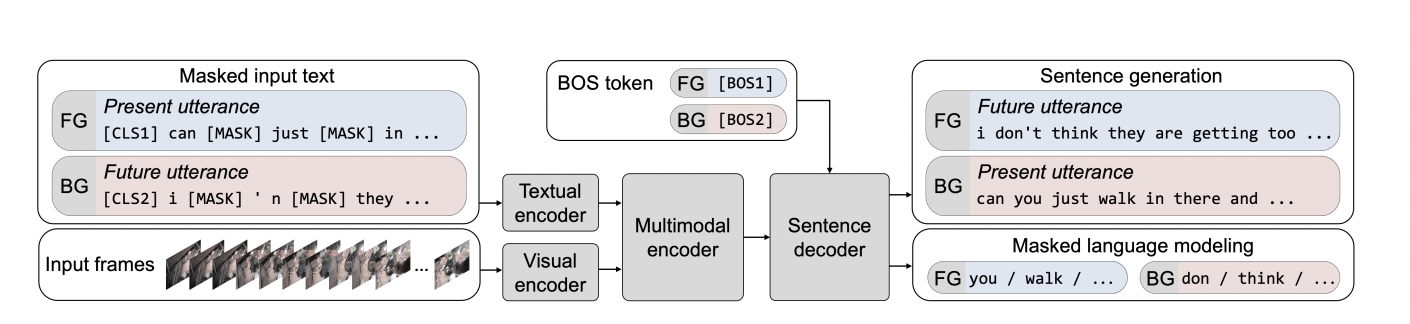
\includegraphics[width=11.6cm]{fig1}
\caption{Multimodal Video Generative Pretraining (MV-GPT) framework. \textbf{BG:} Backward generation, \textbf{FG:} Forward generation}



\end{figure}

\paragraph{}To alleviate the issue of future utterances being temporally unaligned, 
the paper proposes a backward generation objective, where present aligned utterances are 
generated given future utterances. 

\paragraph{}The paper's experimental results show that a model pretrained with this
bidirectional generation objective effectively transfers to multimodal video captioning
and largely outperforms the state of the art.

\paragraph{Method:} The paper's framework aims to take advantage of unlabelled instructional video data,
consisting of video frames and utterances often linked to the visual content.

\paragraph{}The framework requires two textual streams --- input to the encoder and a captioning target
for the decoder. Unlabelled videos do not have captioning targets, so they propose a simple
objective --- the model is trained to generate a \emph{future} utterance in the video given the current
video context and current utterances (forward generation). 

\paragraph{}This allows the model to learn how to optimally fuse modalities in the video encoder,
while the decoder is tasked with predicting a new utterance it has never seen before.

\paragraph{}The paper reiterates, however, that the goal is video captioning, and not "predicting
the future".

\paragraph{}To enable the model to generate text corresponding to the present video context, an
additional backward generation loss is added --- where the model must generate the current utterance given the 
current video frames and a future utterance (backward generation).

\paragraph{}This allows generated sentences to be temporally aligned (and hence more tightly coupled) with 
the visual inputs.

\paragraph{Bi-directional Utterance Generation}

\paragraph{}Given a large set of unlabelled videos, the authors extract short clips
consisting of visual frames $F = \{f_1 ,\ldots, f_{N_f}\}$ and transcribed speech utterances
$U = \{u_1, \ldots, u_{N_u}\}$ aligned with $F$.

\paragraph{}The immediate future utterance $W = \{w_1, \ldots, w_{N_w}\}$, is also considered,
where $u_i$, $w_j$ are the tokenized words in the transcribed utterances. 'Utterances' refer
to a single sentence of transcribed speech.

\paragraph{Forward Generation:} The model is trained to generate a future utterance $W$ given
clip frames $F$ and present utterances $U$. Formally speaking, the formulation for
the forward generation objective to minimize negative log-likelihood of the true future
utterance $W$, where loss given by the chain rule is 
\[
    L_{FG} = -\sum_{i=1}^{N_w} \log P(w_i | w_1,\ldots,w_{i-1}, F, U)
\]

\paragraph{Note:}The visual input $F$ is temporally aligned with the decoder output $U$. This loss
functions encourages the network to generate a caption related to the visual contents.

\paragraph{Backward Generation:} The model applies the same loss as forward generation, now in the 
backward direction. The model is tasked with generating present utterances $U$ aligned with video frames
$F$, conditioned on future utterances $W$ and $F$. Like in forward generation, the following negative
log-likelihood of true present utterance is minimized:

\[
    L_{BG} = -\sum_{i=1}^{N_u}log P(u_i | u_1,\ldots , u_{i-1}, F, W) 
\]

\paragraph{Note:}The visual input $F$ is temporally aligned with the decoder output $U$. This loss function
encourages the network to generate captions related to the visual contents.

\paragraph{Masked Language Modeling:} The model uses masked language modeling as an additional
supplementary loss $L_{MLM}(X)$, where $X$ is the input utterance on which the masking is applied.
This loss is applied on both the forward and backward input utterances, i.e. as 
$L_{MLM}(U)$ and $L_{MLM}(W)$. These losses are computed independently from the above bidirectional
generation losses. 

\paragraph{Model:} The MV-GPT model consists entirely of transformer blocks, and is trained
end-to-end directly from pixels and word tokens.

\paragraph{Modality Specific Encoders:}Given a multimodal video input consisting of the visual frames $F = \{f_1, \ldots, f_{N_f}\}$,
and text inputs $X = \{x_1, \ldots, x_{N_x}\}$, the model first extracts feature from the individual
modalities independently. The textual input $X$ is the aligned utterance $U$ in general (for computing
forward generation loss and for downstream captioning tasks) but is set to $W$ when computing the
backward generation loss.
\paragraph{Textual Encoder:}$N_x$ textual embeddings, $E = \{e_i\}$, are extracted from the input
text using a BERT encoder.
\paragraph{Visual Encoder:}Visual features are extracted directly from pixels, using the transformer-based
encoder ViViT, in particular, the tubelet embedding scheme and the factorized encoder architecture.

\paragraph{}For the tubelet embedding scheme, the spatio-temporal 3D tubes from the visual 
input volume are extracted first, resulting in $S x T$ token embeddings where $S$ and $T$ correspond to 
the number of tokens in the spatial and temporal dimensions respectively.

\paragraph{}The spatial transformer then takes each group of $S$ embeddings from the same temporal
index with a special \emph{CLS} token embedding, and the temporal transformer models interactions
between the output \emph{CLS} embeddings of the individual spatial groups with another \emph{CLS}
embedding resulting in $T+1$ visual features $V = \{v_j\}$.

\paragraph{}Unlike 3D CNN visual encoders, which operate on consecutive frames extracted at high frame
rates (30 fps), this paper's visual encoder can operate on coarsely sampled frames (1 fps), significantly
reducing compute. This allows the model to train the visual encoder end-to-end, and helps it adapt
features across domain gaps between pretraining and downstream datasets. It also allows the easy adoption
of off-the-shelf video augmentation directly to RGB frames, which is useful for small-scale downstream 
benchmarks.

\paragraph{Multimodal Encoder:}Once the two sets of textual features $E$ and visual features $V$ are 
extracted, the model's multimodal encoder fuses multimodal information using a co-attentional transformer.

\paragraph{}Each layer consists of two streams where each stream is a stack of two transformer blocks.
In the textual stream, features $E$ are contextualized using a cross-attention transformer block 
attending to the visual features $V$.

\paragraph{}The output is then further contextualized by another transformer block with self-attention.
The first transformer block performs inter-modality contextualization through a cross-attention process
whereas the second transformer block carries out intra-modality contextualization through a self-attention
process. 

\paragraph{}In the same way, the visual stream $V$ attends to the textual stream. 

\paragraph{}The multimodal encoder repeats this process $R$ times, resulting in the output
multimodal features $\hat{E}$ and $\hat{V}$.
\paragraph{Sentence Decoder:}Given multimodal video features $C = \hat{E} \cup \hat{V}$ as context, 
the model autoregressively generates the output sentence $Y$ conditioned on this context using a 
transformer decoder. To generate token $y_i$, the previously generated tokens $Y_i = \{y_0, \ldots, y_{i-1}\}$
are encoded using a look-up table and a positional embedding to produce $H_i = \{h_0,\ldots, h_{i-1}\}$.

\paragraph{}The context $C$ and the previously embedded tokens $H_i$ are encoded using a single
transformer. The output of this transformer is $\tilde{C} \cup \tilde{H}_i$, where 
$\tilde{H}_i = \{\tilde{h}_0, \ldots, \tilde{h}_{i-1}\}$. 

\paragraph{}$\tilde{C}$ refers to the multimodal input embeddings obtained from the decoder and issue
used for computing the MLM loss.

\paragraph{}The next token $y_i$ is then predicted from $h_{i-1}$ by a linear projection with a softmax:

\[
    y_i = \text{argmax(softmax(}\Phi \tilde{h}_{i-1}))
\]

\paragraph{}where $\Phi \in \mathbb{R}^{v x d}$ is the linear projection matrix and $v$ is the vocabulary
size. The first word $h_0$ is set using a special beginning of sentence (BOS) token. Tokens are 
generated until a special end of sentence (EOS) token is generated.

\paragraph{}In practice, each iteration requires only a single forward pass on the decoder transformer
with the aid of causal masking.

\paragraph{Input and Output Configurations}

\paragraph{Pretraining:} The pretraining objective is bidirectional. As such, 
the triplets ($F, U, W)$ consisting
of the visual frames $F$, present utterances $U$, and the future utterance $W$ are processed by the network
twice.  

\paragraph{}For forward generation, the model takes $F$ and $U$ as inputs and generates $W$, and it 
generates $W$.

\paragraph{}In backward generation, the model generates $U$ given $F$ and $W$.

\paragraph{}To enable the model to recognize the different configurations, distinct tokens CLS1, and CLS2
are attached to the input text for the forward and backward generation losses respectively. Similarly,
BOS1 and BOS2 tokens are fed to the decoder to initiate sentence generation.

\paragraph{Finetuning for Captioning:}With downstream video captioning datasets, video clips (consisting of 
frames $F$ and aligned utterances $U$) are manually annotated with a natural language caption.

\paragraph{}During finetuning, CS1 tokens are attached to $U$ (as is done in forward generation),
since $U$ is an aligned utterance. However, for generation, the model is fed BOS2 tokens (
as is done in backward generation to predict present utterances), so as to generate a temporally
aligned caption.

\paragraph{Implementation Details:}The authors of this paper adopted the BERT-Base architecture
with uncased wordpiece tokenization. The model's visual encoder uses the corresponding 
ViViT-Base configuration with a 1-layer temporal transformer and tubelet size of 16x16x4.

\paragraph{}The model's multimodal encoder consists of 2 layers and finally the decoder itself
is based on GPT-2 (with 117M parameters). The authors modify GPT-2 to take both multimodal
input context $C$ and a BOS token, allowing conditional generation (the original GPT starts
generation immediately by taking the first word as its input and only conditions on text).

\paragraph{}The text encoder and decoder are initialized with the standard BERT and GPT-2 wieghts
respectively, pretrained on large-scale unlabelled corpora.

\paragraph{}The visual encoder is initialized using pretrained weights on Kinetics 400.

\paragraph{}The model is pretrained end-to-end using the Adam optimizer for 1.5M iterations with
batch size 2048. 

\paragraph{Results:} See Table 1, 2.

\begin{figure}
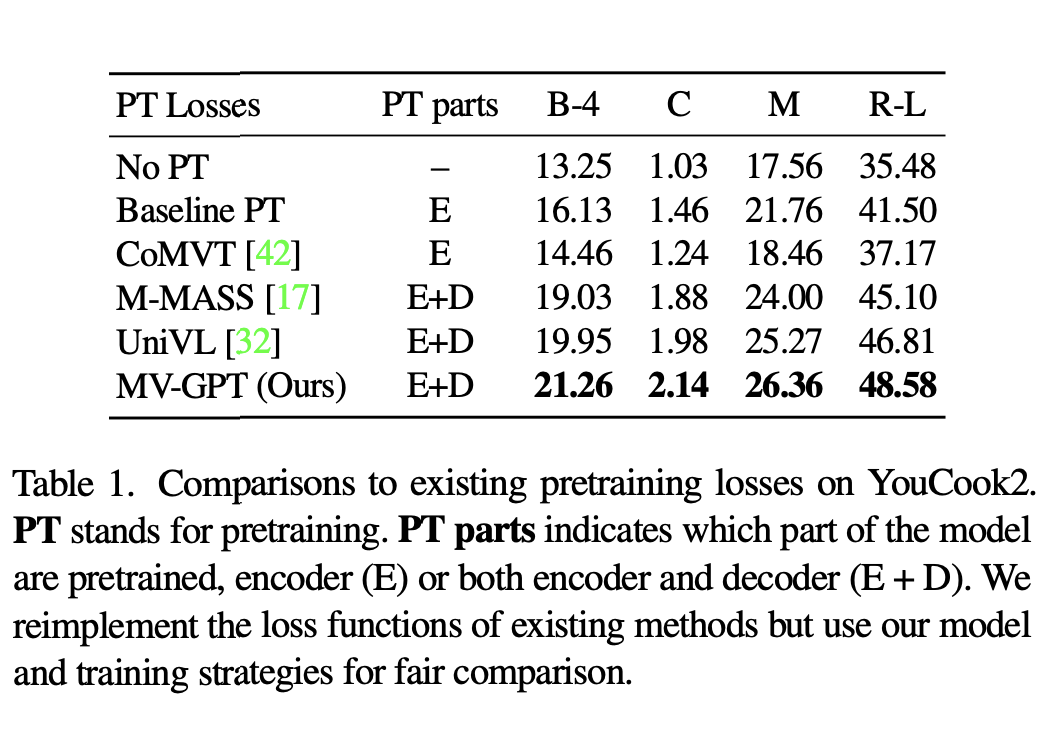
\includegraphics[width=8cm]{fig2}
\centering
\end{figure}



\begin{figure}
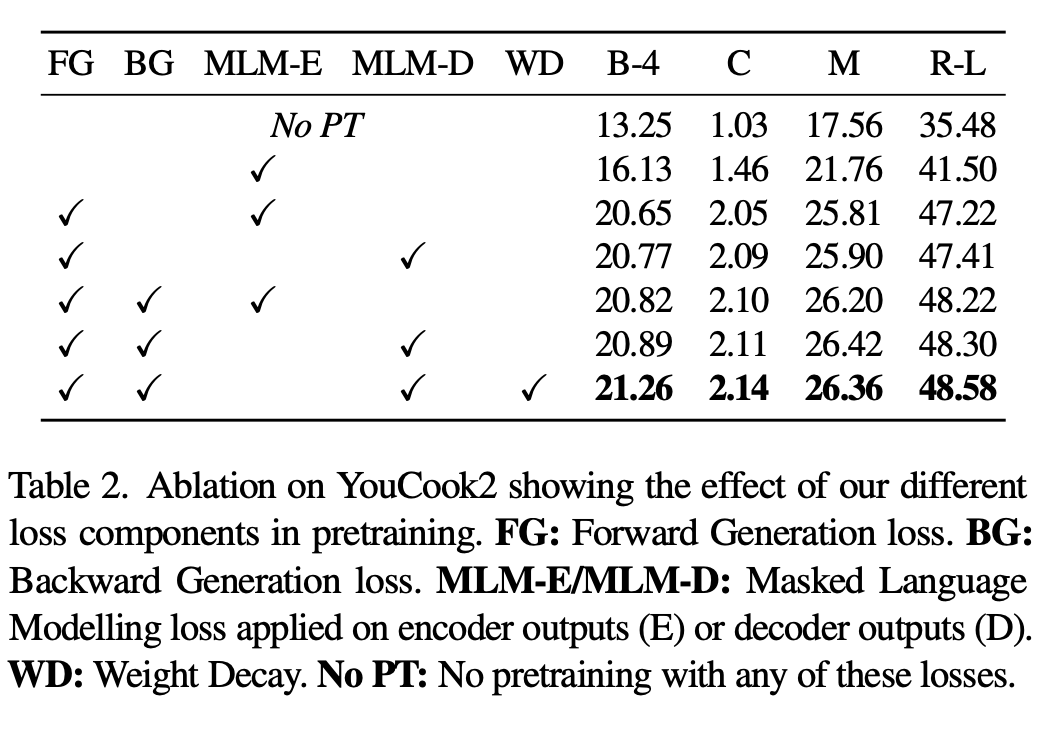
\includegraphics[width=8cm]{fig3}
\centering
\end{figure}

\end{document}
